% Options for packages loaded elsewhere
\PassOptionsToPackage{unicode}{hyperref}
\PassOptionsToPackage{hyphens}{url}
\PassOptionsToPackage{dvipsnames,svgnames,x11names}{xcolor}
%
\documentclass[
  letterpaper,
  DIV=11,
  numbers=noendperiod]{scrartcl}

\usepackage{amsmath,amssymb}
\usepackage{iftex}
\ifPDFTeX
  \usepackage[T1]{fontenc}
  \usepackage[utf8]{inputenc}
  \usepackage{textcomp} % provide euro and other symbols
\else % if luatex or xetex
  \usepackage{unicode-math}
  \defaultfontfeatures{Scale=MatchLowercase}
  \defaultfontfeatures[\rmfamily]{Ligatures=TeX,Scale=1}
\fi
\usepackage{lmodern}
\ifPDFTeX\else  
    % xetex/luatex font selection
\fi
% Use upquote if available, for straight quotes in verbatim environments
\IfFileExists{upquote.sty}{\usepackage{upquote}}{}
\IfFileExists{microtype.sty}{% use microtype if available
  \usepackage[]{microtype}
  \UseMicrotypeSet[protrusion]{basicmath} % disable protrusion for tt fonts
}{}
\makeatletter
\@ifundefined{KOMAClassName}{% if non-KOMA class
  \IfFileExists{parskip.sty}{%
    \usepackage{parskip}
  }{% else
    \setlength{\parindent}{0pt}
    \setlength{\parskip}{6pt plus 2pt minus 1pt}}
}{% if KOMA class
  \KOMAoptions{parskip=half}}
\makeatother
\usepackage{xcolor}
\setlength{\emergencystretch}{3em} % prevent overfull lines
\setcounter{secnumdepth}{5}
% Make \paragraph and \subparagraph free-standing
\ifx\paragraph\undefined\else
  \let\oldparagraph\paragraph
  \renewcommand{\paragraph}[1]{\oldparagraph{#1}\mbox{}}
\fi
\ifx\subparagraph\undefined\else
  \let\oldsubparagraph\subparagraph
  \renewcommand{\subparagraph}[1]{\oldsubparagraph{#1}\mbox{}}
\fi


\providecommand{\tightlist}{%
  \setlength{\itemsep}{0pt}\setlength{\parskip}{0pt}}\usepackage{longtable,booktabs,array}
\usepackage{calc} % for calculating minipage widths
% Correct order of tables after \paragraph or \subparagraph
\usepackage{etoolbox}
\makeatletter
\patchcmd\longtable{\par}{\if@noskipsec\mbox{}\fi\par}{}{}
\makeatother
% Allow footnotes in longtable head/foot
\IfFileExists{footnotehyper.sty}{\usepackage{footnotehyper}}{\usepackage{footnote}}
\makesavenoteenv{longtable}
\usepackage{graphicx}
\makeatletter
\def\maxwidth{\ifdim\Gin@nat@width>\linewidth\linewidth\else\Gin@nat@width\fi}
\def\maxheight{\ifdim\Gin@nat@height>\textheight\textheight\else\Gin@nat@height\fi}
\makeatother
% Scale images if necessary, so that they will not overflow the page
% margins by default, and it is still possible to overwrite the defaults
% using explicit options in \includegraphics[width, height, ...]{}
\setkeys{Gin}{width=\maxwidth,height=\maxheight,keepaspectratio}
% Set default figure placement to htbp
\makeatletter
\def\fps@figure{htbp}
\makeatother
% definitions for citeproc citations
\NewDocumentCommand\citeproctext{}{}
\NewDocumentCommand\citeproc{mm}{%
  \begingroup\def\citeproctext{#2}\cite{#1}\endgroup}
\makeatletter
 % allow citations to break across lines
 \let\@cite@ofmt\@firstofone
 % avoid brackets around text for \cite:
 \def\@biblabel#1{}
 \def\@cite#1#2{{#1\if@tempswa , #2\fi}}
\makeatother
\newlength{\cslhangindent}
\setlength{\cslhangindent}{1.5em}
\newlength{\csllabelwidth}
\setlength{\csllabelwidth}{3em}
\newenvironment{CSLReferences}[2] % #1 hanging-indent, #2 entry-spacing
 {\begin{list}{}{%
  \setlength{\itemindent}{0pt}
  \setlength{\leftmargin}{0pt}
  \setlength{\parsep}{0pt}
  % turn on hanging indent if param 1 is 1
  \ifodd #1
   \setlength{\leftmargin}{\cslhangindent}
   \setlength{\itemindent}{-1\cslhangindent}
  \fi
  % set entry spacing
  \setlength{\itemsep}{#2\baselineskip}}}
 {\end{list}}
\usepackage{calc}
\newcommand{\CSLBlock}[1]{\hfill\break\parbox[t]{\linewidth}{\strut\ignorespaces#1\strut}}
\newcommand{\CSLLeftMargin}[1]{\parbox[t]{\csllabelwidth}{\strut#1\strut}}
\newcommand{\CSLRightInline}[1]{\parbox[t]{\linewidth - \csllabelwidth}{\strut#1\strut}}
\newcommand{\CSLIndent}[1]{\hspace{\cslhangindent}#1}

\KOMAoption{captions}{tableheading}
\makeatletter
\@ifpackageloaded{caption}{}{\usepackage{caption}}
\AtBeginDocument{%
\ifdefined\contentsname
  \renewcommand*\contentsname{Table of contents}
\else
  \newcommand\contentsname{Table of contents}
\fi
\ifdefined\listfigurename
  \renewcommand*\listfigurename{List of Figures}
\else
  \newcommand\listfigurename{List of Figures}
\fi
\ifdefined\listtablename
  \renewcommand*\listtablename{List of Tables}
\else
  \newcommand\listtablename{List of Tables}
\fi
\ifdefined\figurename
  \renewcommand*\figurename{Figure}
\else
  \newcommand\figurename{Figure}
\fi
\ifdefined\tablename
  \renewcommand*\tablename{Table}
\else
  \newcommand\tablename{Table}
\fi
}
\@ifpackageloaded{float}{}{\usepackage{float}}
\floatstyle{ruled}
\@ifundefined{c@chapter}{\newfloat{codelisting}{h}{lop}}{\newfloat{codelisting}{h}{lop}[chapter]}
\floatname{codelisting}{Listing}
\newcommand*\listoflistings{\listof{codelisting}{List of Listings}}
\makeatother
\makeatletter
\makeatother
\makeatletter
\@ifpackageloaded{caption}{}{\usepackage{caption}}
\@ifpackageloaded{subcaption}{}{\usepackage{subcaption}}
\makeatother
\ifLuaTeX
  \usepackage{selnolig}  % disable illegal ligatures
\fi
\usepackage{bookmark}

\IfFileExists{xurl.sty}{\usepackage{xurl}}{} % add URL line breaks if available
\urlstyle{same} % disable monospaced font for URLs
\hypersetup{
  pdftitle={T is for Topology},
  pdfauthor={Tanya Strydom; Andrew P. Beckerman},
  pdfkeywords={food web, network construction},
  colorlinks=true,
  linkcolor={blue},
  filecolor={Maroon},
  citecolor={Blue},
  urlcolor={Blue},
  pdfcreator={LaTeX via pandoc}}

\title{T is for Topology}
\author{Tanya Strydom \and Andrew P. Beckerman}
\date{2024-03-19}

\begin{document}
\maketitle
\begin{abstract}
There are many reasons one might want to generate a network and there
are many tools on the market that might make that possible. However not
all tools are created equally and there is reason to assume that not all
networks will suit most purposes. Here the aim is to compare and
contrast the different topology generating tools that are on the market
and see where they shine and where they fall flat. There probably isn't
one model to rule them all but it doesn't mean that we shouldn't be
critical when we think about the model we want to use.
\end{abstract}

\section{Introduction}\label{introduction}

\begin{itemize}
\item
  In order to construct a `perfect' network \emph{i.e.,} one which
  \emph{perfectly} captures the dynamics for a specific community one
  needs to consider and account for many different moving parts
  (\emph{e.g.,}). So when developing a model it makes sense that you
  prioritise the aspect of the prediction/construction task that has the
  most value for your research goal, acknowledging that a model might
  fall short in others. The thing is that with the growing suite of
  approaches to generating networks it is important that we don't lose
  sight of the core philosophy behind the model we use and to ensure
  that we are using the model best suited to what we want to be
  accomplishing.
\item
  It is perhaps useful to start with asking why do we want/need models
  to generate networks. This can be broadly thought of to fall into two
  categories. Build networks because we want to build concepts vs build
  networks because we want specificity. Broadly this means that we
  either want to construct/predict a collection of interactions
  (generate networks) or a network of interactions (predict
  interactions).
\end{itemize}

Arguably the need for methods and tools for constructing interaction
networks arises from two different (but still aligned) places of
interest within the field of network ecology. On the one side sits the
researcher who is interested in generating a set of ecologically
plausible but not necessarily realised `in the field' networks for the
purpose of running further simulations (\emph{e.g.,} extinction sim
\textbf{TODO}) or understanding some higher-level process/concept
(\emph{e.g.,} energetics \textbf{TODO}). This researcher is contrasted
by one that is interested in constructing real-world, location specific,
interaction data in lieu of inventorying interactions based n
observations made in the field (Strydom et al. 2021). Of course these
two categories are not two distinct, mutually exclusive, groups but can
rather be viewed as operating on a gradient ranging from a need for
generality (\emph{i.e.,} creating a network that, when taken in
aggregate, the distribution of links (interactions) between species are
ecologically plausible) to a need for specificity (local-level
predictions between specific species).

\begin{itemize}
\item
  A breakdown of network generators; statement of need and core
  philosophies
\item
  A breakdown of interaction predictors; statement of need ((Jordano
  2016b, 2016a; Poisot et al. 2021)) and core philosophies
  (trait-matching, coexistence)
\item
  Stands to reason then that we have developed methods specialise in one
  or the other. Which comes at a cost of `performance' in other aspects.
  Knowing how the different model families stack up to each other is
  thus valuable and that is kinda what we are trying to achieve.
\end{itemize}

Joel E. Cohen, Newman, and Steele (1985) states that \emph{``{[}Their{]}
approach is more like gross anatomy than like physiology\ldots{} that
is, the gross anatomy is frozen, rather than in motion.''}.

Interestingly Williams and Martinez (2008) also explicitly talk about
\emph{structural} food-web models in their introduction\ldots{} so how I
see it that means that there has always been this inherent
acknowledgement that models are functioning at a specific `network
level'.

\subsection{The history behind the
approach}\label{the-history-behind-the-approach}

Maybe a brief history of the development of predictive tools/topo
generators? Sort of where the theory/body of work was based and how that
has changed? IS there a difference between topo generator and predictive
tool - I'm inclined to think that it aligns with the whole debate of
high level structure vs node-level perfection

Maybe start here with discussing the core mechanistic differences that
models will work at --- some are really concerned about (and thus
constrained by) structure, others are more mechanistic in nature
\emph{i.e.,} species \emph{a} has the capacity to eat species \emph{b}
because traits (read gob size), and then you get Rohr et al. (2010) and
Strydom et al. (2022) that sit in the weird liminal latent space\ldots{}

Here I will probably get on my (newly discovered) soapbox and wax
lyrical about how in certain situations structure is enough (and that
will probably be for some high-level things like thinking about energy
flows etc., I can also see a world in which maybe you want to do some
sort of robustness/extinction work - since then you're usually doing
`random' (within limits) extinctions) but there may be use cases where
we are really interested in the node-level interactions \emph{i.e.,}
species identity is like a thing we need to care about and also be able
to retrieve specific interactions at specific nodes correctly. What is
the purpose of generating a network? Is it an element of a bigger
question we are asking, \emph{e.g.,} I want to generate a series of
networks to do some extinction simulations/bioenergetic stuff OR are we
looking for a `final product' network that is relevant to a specific
location? (this can still be broad in geographic scope).

At some point we are going to need to discuss the key differences and
implications between predicting a metaweb (\emph{sensu} Jennifer A.
Dunne (2006)) and a network realisation. And here I can't help but think
about Poisot, Stouffer, and Gravel (2015) (and probably other papers)
that discuss how the local factors are going to play a role and even the
same pair of species may interact differently in different points in the
landscape.

\begin{quote}
Do we need to delve into individual-based networks? (\emph{sensu} Tinker
2012, Araújo 2008) I think its probably a step too far and one starts
creeping into apples and pears type of comparisons. Especially since
these work off of already existing networks (I seem to recall) and its
more about about `tweaking' those - so not so much \emph{de novo}
predictions. Although this might be useful to keep in mind when it comes
to re-wiring\ldots{} Also on that note do we opn the re-wiring door here
in this ms or wait it out a bit.
\end{quote}

\section{Data \& Methods}\label{sec-data-methods}

Here we only look at families of models that are explicitly developed to
construct \emph{de novo} networks, be this in the form of either
artificial or synthetic networks.

\subsection{Topology Generators}\label{topology-generators}

\textbf{Null models} (Erdős and Rényi 1959): Links are assembled
randomly, not developed within an ecological framework. But of course
could still hold if we assume that communities are randomly assembled in
terms of who is interacting with who (I seem to think that's sort of
what May was arguing but I would need to remind myself)

\textbf{Neutral models}

\textbf{Cascade model} (Joel E. Cohen, Briand, and Newman 1990): Much
like the name suggests the cascade model rests on the idea that species
feed on one another in a hierarchical manner. This rests on the
assumption that the links within a network are variably distributed
across the network; with the proportion of links decreasing as one moves
up the trophic levels (\emph{i.e.,} `many' prey and `few' predators).
This is achieved by assigning all species a random rank, this rank will
then determine both the predators and prey of that species. A species
will have a particular probability of being fed on by any species with a
higher ranking than it, this probability is constrained by the specified
connectance of the network. Interestingly here `species' are treated as
any individual that consume and are consumed by the same `species',
\emph{i.e.,} these are not taxonomical species (Joel E. Cohen, Newman,
and Steele 1985). The original cascade model has altered to be more
`generalised' (Stouffer et al. 2005), which altered the probability
distribution of the prey that could be consumed by a species.

\textbf{Niche models} (Williams and Martinez 2000): The niche model
introduces the idea that species interactions are based on the `feeding
niche' of a species. Broadly, all species are randomly assigned a
`feeding niche' range and all species that fall in this range can be
consumed by that species (thereby allowing for cannibalism). The niche
of each species is randomly assigned and the range of each species'
niche is (in part) constrained by the specified connectance of the
network. The niche model has also been modified, although it appears
that adding to the `complexity' of the niche model does not improve on
its ability to generate a more ecologically `correct' network (Williams
and Martinez 2008).

\textbf{Nested hierarchy model} (Cattin et al. 2004):

\begin{quote}
Gravel et al. (2013) also poses an interesting cross-over between the
adbm and niche model.
\end{quote}

\subsection{Interaction Predictors}\label{interaction-predictors}

\textbf{Allometric diet breadth model (ADBM)} (Petchey et al. 2008):
``Our modelling effort therefore asks how well our model can predict the
arrangement rather than the number of feeding links in food webs.'' This
is a scaled version of the diet breadth model (Beckerman, Petchey, and
Warren 2006)

\textbf{Log-ratio} (Rohr et al. 2010): Interestingly often used in paleo
settings (at least that's what it currently looks like in my
mind\ldots{} Pires et al. (2020))

\textbf{Matching} (Rossberg et al. 2006): This one is more of a dynamic
model (so BEF) and maybe beyond the scope of this work. I think there is
value on only focusing on the `static' models at this point (probably
have said this before elsewhere but yeah)

\textbf{PFIM} (Shaw et al. 2024):

\textbf{Trait-based} (Caron et al. 2022):

\textbf{Graph embedding} (Strydom et al. 2022, 2023): At a high level
graph embedding focuses on capturing the structural data of a network as
opposed to a list of pairwise (\emph{i.e.,} mechanistic) interactions.
Here specifically the embedding is preformed on a known interaction
network and captures information as to where species (nodes) are
positioned in a network \emph{e.g.,} are they basal prey species or top
predators, similar to the log ratio model. In Strydom et al. (2022) the
products of the embedding process are fed into a transfer learning
framework for novel prediction\ldots{}

I know tables are awful but in this case they may make more sense. Also
I don't think I'm at the point where I can say that the table is
complete/comprehensive but it getting there Not sure about putting in
some papers that have used the model - totes happy to drop those I
think\ldots{}

\begin{longtable}[]{@{}
  >{\raggedright\arraybackslash}p{(\columnwidth - 10\tabcolsep) * \real{0.1667}}
  >{\raggedright\arraybackslash}p{(\columnwidth - 10\tabcolsep) * \real{0.1667}}
  >{\raggedright\arraybackslash}p{(\columnwidth - 10\tabcolsep) * \real{0.1667}}
  >{\raggedright\arraybackslash}p{(\columnwidth - 10\tabcolsep) * \real{0.1667}}
  >{\raggedright\arraybackslash}p{(\columnwidth - 10\tabcolsep) * \real{0.1667}}
  >{\raggedright\arraybackslash}p{(\columnwidth - 10\tabcolsep) * \real{0.1667}}@{}}
\caption{Lets make a table that gives an overview of the different
topology generators that we will look at. Here I take `data-driven' to
refer to the need for `real world' data. This can probably be approached
in a different way though maybe?}\label{tbl-history}\tabularnewline
\toprule\noalign{}
\begin{minipage}[b]{\linewidth}\raggedright
Model
\end{minipage} & \begin{minipage}[b]{\linewidth}\raggedright
Core Mechanism
\end{minipage} & \begin{minipage}[b]{\linewidth}\raggedright
Predicts
\end{minipage} & \begin{minipage}[b]{\linewidth}\raggedright
Specificity
\end{minipage} & \begin{minipage}[b]{\linewidth}\raggedright
Interaction
\end{minipage} & \begin{minipage}[b]{\linewidth}\raggedright
Data-driven
\end{minipage} \\
\midrule\noalign{}
\endfirsthead
\toprule\noalign{}
\begin{minipage}[b]{\linewidth}\raggedright
Model
\end{minipage} & \begin{minipage}[b]{\linewidth}\raggedright
Core Mechanism
\end{minipage} & \begin{minipage}[b]{\linewidth}\raggedright
Predicts
\end{minipage} & \begin{minipage}[b]{\linewidth}\raggedright
Specificity
\end{minipage} & \begin{minipage}[b]{\linewidth}\raggedright
Interaction
\end{minipage} & \begin{minipage}[b]{\linewidth}\raggedright
Data-driven
\end{minipage} \\
\midrule\noalign{}
\endhead
\bottomrule\noalign{}
\endlastfoot
random & random & networks & species agnostic & binary & no \\
cascade & structural & networks & species agnostic & binary & no \\
niche & structural & networks & species agnostic & binary & no \\
nested hierarchical & structural & networks & species agnostic & binary
& no \\
ADBM & mechanistic & interactions & energetics & quantitative & \\
log-ratio & & interactions & & & \\
PFIM & mechanistic & interactions & trait based & & \\
graph embedding & embedding & interactions & evolutionary &
probabilistic & yes \\
trait model & mechanistic & interactions & trait based & & yes \\
matching & & & & & \\
\end{longtable}

\begin{quote}
Might be nice to have a little appendix/supp mat that breaks down the
models in detail so that they are all in one place so that someone (grad
student being told they need to build networks) some day can go and
educate themselves with slightly lower effort. This will also be useful
for me should I end up having to do some actual coding - think of this
as step one in the pseudo code process.
\end{quote}

\subsection{Datasets used}\label{datasets-used}

Here I think we need to span a variety of domains, at minimum aquatic
and terrestrial but maybe there should be a `scale' element as well
\emph{i.e.,} a regional and local network. I think there is going to be
a `turning point' where structural will take over from mechanistic in
terms of performance. More specifically at local scales bioenergetic
constraints (and co-occurrence) may play a bigger role in structuring a
network whereas at the metaweb level then mechanistic may make more
(since by default its about who can potentially interact and obviously
not constrained by real-world scenarios) \emph{sensu} Caron et al.
(2023). Although having said that I feel that contradicts the idea of
backbones (\emph{sensu} Bramon Mora (sp?) et al \& Stouffer et al) But
that might be where we get the idea of core \emph{structure} vs
something like linkage density. So core things like trophic level/chain
length will be conserved but connectance might not (I think I understand
what I'm trying to say here)

I think we should also use the Dunne (I think) Cambrian (also think)
network (I was correct and its this one Jennifer A. Dunne et al.
(2008)). Because 1) it gives the paleo-centric methods their moment in
the sun and 2) I think it also brings up the interesting question of can
we use modern structure to predict past ones? Here one might expect a
more mechanistic approach to shine.

Draw the other datasets from \texttt{Mangal} because they will be nicely
formatted and essentially at point and shoot level

\subsection{Comparing different
models}\label{comparing-different-models}

For now the (still essentially pending) workflow/associated code can be
found at the following repository
\href{https://github.com/BecksLab/topology_generators}{BecksLab/topology\_generators}

\begin{enumerate}
\def\labelenumi{\arabic{enumi}.}
\tightlist
\item
  Shortlist/finalise the different topo generators
\item
  collate/translate into \texttt{Julia}

  \begin{itemize}
  \tightlist
  \item
    \emph{e.g.,} some models wil be in SpeciesInteractionNetworks.jl
    (new EcoNet); I know (parts of) the transfer learning stuff is and
    the niche model
  \item
    others will need to be coded out (the more simpler models should be
    easier)
  \item
    can also consider \texttt{R} but then it becomes a case of porting
    things left and right depending on how we decide to do the post
    analyses
  \end{itemize}
\item
  Curate networks for the different datasets/scenarios we select - I
  feel like there might be some scenarios that we can't do all models
  for all datasets but maybe I'm being a pessimist.

  \begin{itemize}
  \tightlist
  \item
    Need to also think about where one might find the additional data
    for some of the models\ldots{}

    \begin{itemize}
    \tightlist
    \item
      Body size: Herberstein et al. (2022) - Although maybe Andrew has
      strong thotsTM RE the one true body size database to rule them
      all\ldots{}
    \item
      Other trait sources: Wilman et al. (2014) and Jones et al. (2009)
    \item
      This is where we'll get the paleo traits from if I'm correct
      Bambach, Bush, and Erwin (2007)
    \item
      Phylogeny stuff: Upham, Esselstyn, and Jetz (2019) (what we used
      for TL but its only mammals\ldots) but I'm sure there will be
      others
    \end{itemize}
  \item
    Also limitation of scope\ldots{} \emph{e.g.,} do we even dare to
    think about including plants/basal producers (see \emph{e.g.,}
    Valdovinos et al. (2023))
  \item
    Taxonomic harmonisation - something to think about and check
  \end{itemize}
\item
  compare model performance based on the ideas currently listed in the
  results section.
\item
  Make a pretty picture that summarises things - maybe overlapping Venn
  circles that showcase which models do well in the different
  spheres/aspects of life
\end{enumerate}

\section{Results}\label{results}

How we want to compare and contrast. I think there won't be a `winner'
and thus we need to think of `tests' that are going to measure
performance in different situations/settings. With that in mind I think
some valuable points to consider would be:

\begin{itemize}
\tightlist
\item
  Structural vs pairwise link predictions (graph vs node level)

  \begin{itemize}
  \tightlist
  \item
    \% of links correctly retrieved
  \item
    connectance
  \item
    trophic level
  \item
    generalism vs specialism
  \item
    something related to false positives/negatives
  \item
    intervality
  \end{itemize}
\item
  Data `cost' (some methods might need a lot lot of supporting data vs
  something very light weight)
\item
  I think it would be remiss to not also take into consideration
  computational cost
\item
  something about the network output - I'm acknowledging my biases and
  saying that probabilistic (or \emph{maybe} weighted) links are the way
\end{itemize}

Joel E. Cohen, Newman, and Steele (1985) actually tells us that the
cascade model only really works for communities that range from 3-33
species\ldots{} and Williams and Martinez (2008) also highlights how
structural models really only work for small communities

\begin{quote}
maybe we can put these into broader categories - if we do start doing
the venn overlap thing. \emph{E.g.,} local scale predictions, regional
scale predictions, pairwise interactions, structural (energetics),
computationally cheap, low cost data
\end{quote}

\subsection{Quantitative stuff}\label{quantitative-stuff}

\begin{figure}[H]

\centering{

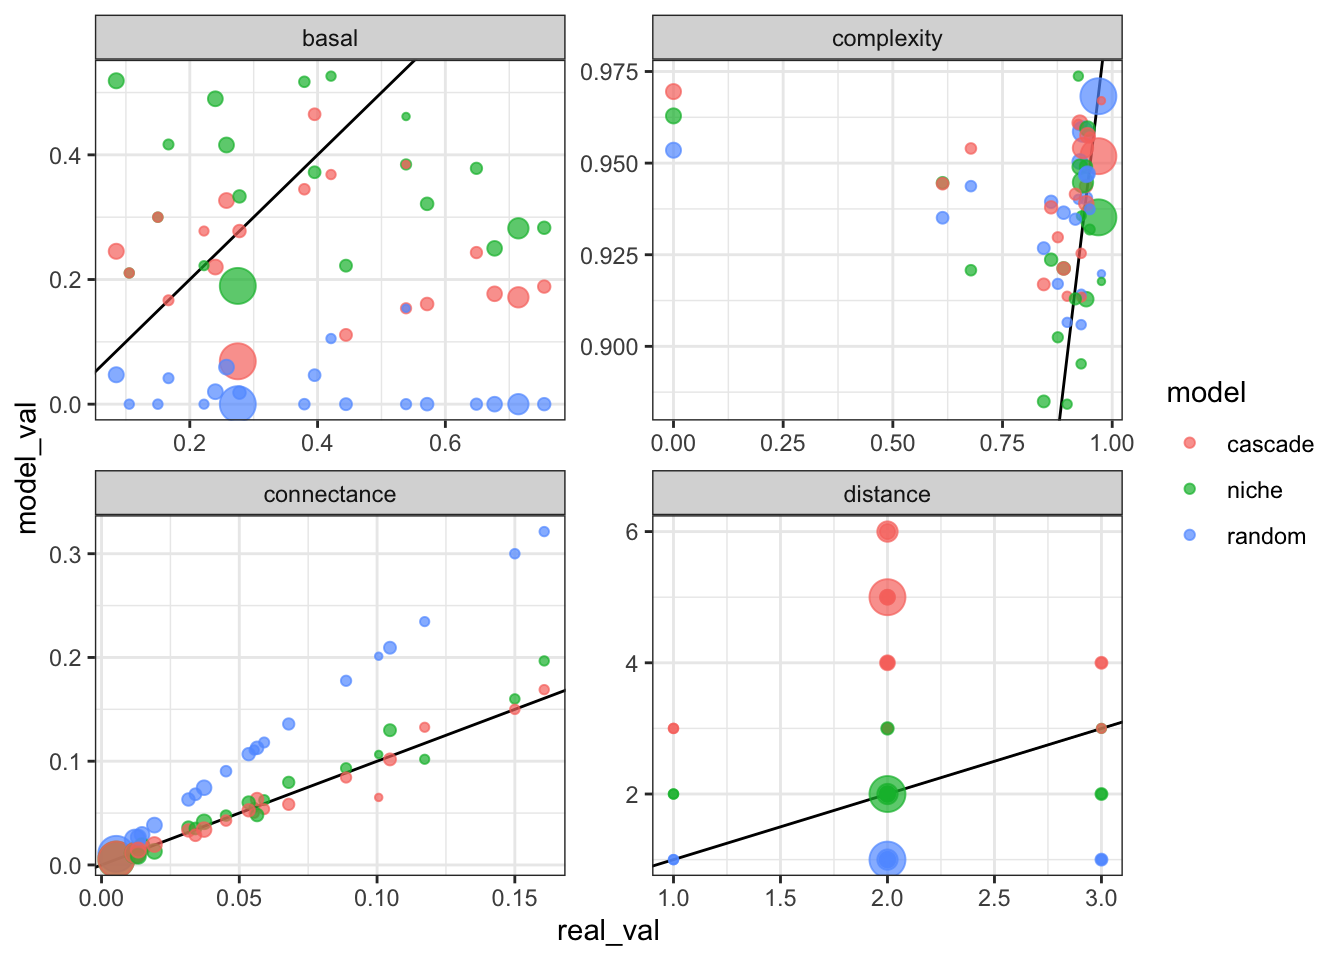
\includegraphics{index_files/figure-latex/notebooks-model_quantitative-fig-topology-output-1.png}

}

\caption{\label{fig-topology}Real vs observed values for network summary
statistics. Note here that `basal' is calculated as the proportion of
species that have a generality value of zero \emph{i.e.,} are basal
AFAIK}

\end{figure}%

\textsubscript{Source:
\href{https://BecksLab.github.io/ms_t_is_for_topology/index.qmd.html}{Article
Notebook}}

This is actually an awful way to try and summarise the data but rolling
with it for now\ldots{}

\section{Discussion}\label{discussion}

I think a big take home will (hopefully) be how different approaches do
better in different situations and so you as an end user need to take
this into consideration and pick accordingly. I think Petchey et al.
(2011) might have (and share) some thoughts on this (thanks Andrew). I
feel like I need to look at Berlow, Brose, and Martinez (2008) but maybe
not exactly in this context but vaguely adjacent.

An interesting thing to also think about (and arguably it will be
addressed based on some of the other thoughts and ideas) is data
dependant and data independent `parametrisation' of the models\ldots{}

I probably think about this point too much but a point of discussion
that I think will be interesting to bring up the idea that if a model is
missing a specific pairwise link but doing well at the structural level
then when does it matter? I think this is covered with the whole node vs
graph level performance but I kind of just want to bring it up here
again because also one of those things that I think about a bit too much
probably\ldots{}

\begin{quote}
Thinking very long term here and maybe a bit beyond the scope but also
thinking about a multi- model approach? So in other words using one
model to build an initial network but maybe a second one to constrain it
a bit better. I blame this thought on the over-connected PFIM food
webs\ldots{}
\end{quote}

\section*{References}\label{references}
\addcontentsline{toc}{section}{References}

\textsubscript{Source:
\href{https://BecksLab.github.io/ms_t_is_for_topology/index.qmd.html}{Article
Notebook}}

\phantomsection\label{refs}
\begin{CSLReferences}{1}{0}
\bibitem[\citeproctext]{ref-bambachAutecologyFillingEcospace2007}
Bambach, Richard K., Andrew M. Bush, and Douglas H. Erwin. 2007.
{``Autecology and the {Filling} of {Ecospace}: {Key Metazoan
Radiations}.''} \emph{Palaeontology} 50 (1): 1--22.
\url{https://doi.org/10.1111/j.1475-4983.2006.00611.x}.

\bibitem[\citeproctext]{ref-beckermanForagingBiologyPredicts2006}
Beckerman, Andrew P., Owen L. Petchey, and Philip H. Warren. 2006.
{``Foraging Biology Predicts Food Web Complexity.''} \emph{Proceedings
of the National Academy of Sciences} 103 (37): 13745--49.
\url{https://doi.org/10.1073/pnas.0603039103}.

\bibitem[\citeproctext]{ref-berlowGoldilocksFactorFood2008}
Berlow, Eric L., Ulrich Brose, and Neo D. Martinez. 2008. {``The
{`{Goldilocks} Factor'} in Food Webs.''} \emph{Proceedings of the
National Academy of Sciences} 105 (11): 4079--80.
\url{https://doi.org/10.1073/pnas.0800967105}.

\bibitem[\citeproctext]{ref-caronTrophicInteractionModels2023}
Caron, Dominique, Ulrich Brose, Miguel Lurgi, Guillaume Blanchet,
Dominique Gravel, and Laura J. Pollock. 2023. {``Trophic Interaction
Models Predict Interactions Across Space, Not Food Webs.''} EcoEvoRxiv.
\url{https://doi.org/10.32942/X29K55}.

\bibitem[\citeproctext]{ref-caronAddressingEltonianShortfall2022}
Caron, Dominique, Luigi Maiorano, Wilfried Thuiller, and Laura J.
Pollock. 2022. {``Addressing the {Eltonian} Shortfall with Trait-Based
Interaction Models.''} \emph{Ecology Letters} 25 (4): 889--99.
\url{https://doi.org/10.1111/ele.13966}.

\bibitem[\citeproctext]{ref-cattinPhylogeneticConstraintsAdaptation2004}
Cattin, Marie-France, Louis-Félix Bersier, Carolin Banašek-Richter,
Richard Baltensperger, and Jean-Pierre Gabriel. 2004. {``Phylogenetic
Constraints and Adaptation Explain Food-Web Structure.''} \emph{Nature}
427 (6977): 835--39. \url{https://doi.org/10.1038/nature02327}.

\bibitem[\citeproctext]{ref-cohenCommunityFoodWebs1990}
Cohen, Joel E, Frederic Briand, and Charles Newman. 1990.
\emph{Community {Food Webs}: {Data} and {Theory}}. Biomathematics.
Berlin Heidelberg: Springer-Verlag.

\bibitem[\citeproctext]{ref-cohenStochasticTheoryCommunity1985}
Cohen, Joel E., C. M. Newman, and John Hyslop Steele. 1985. {``A
Stochastic Theory of Community Food Webs {I}. {Models} and Aggregated
Data.''} \emph{Proceedings of the Royal Society of London. Series B.
Biological Sciences} 224 (1237): 421--48.
\url{https://doi.org/10.1098/rspb.1985.0042}.

\bibitem[\citeproctext]{ref-dunneNetworkStructureFood2006}
Dunne, Jennifer A. 2006. {``The {Network Structure} of {Food Webs}.''}
In \emph{Ecological Networks: {Linking} Structure and Dynamics}, edited
by Jennifer A Dunne and Mercedes Pascual, 27--86. Oxford University
Press.

\bibitem[\citeproctext]{ref-dunneCompilationNetworkAnalyses2008}
Dunne, Jennifer A., Richard J. Williams, Neo D. Martinez, Rachel A.
Wood, and Douglas H. Erwin. 2008. {``Compilation and {Network Analyses}
of {Cambrian Food Webs}.''} \emph{PLOS Biology} 6 (4): e102.
\url{https://doi.org/10.1371/journal.pbio.0060102}.

\bibitem[\citeproctext]{ref-erdosRandomGraphs1959}
Erdős, Paul, and Alfréd Rényi. 1959. {``On {Random Graphs I}.''}
\emph{Publicationes Mathematicae}.
\url{https://doi.org/10.5486/PMD.1959.6.3-4.12}.

\bibitem[\citeproctext]{ref-gravelInferringFoodWeb2013}
Gravel, Dominique, Timothée Poisot, Camille Albouy, Laure Velez, and
David Mouillot. 2013. {``Inferring Food Web Structure from
Predator--Prey Body Size Relationships.''} \emph{Methods in Ecology and
Evolution} 4 (11): 1083--90.
\url{https://doi.org/10.1111/2041-210X.12103}.

\bibitem[\citeproctext]{ref-herbersteinAnimalTraitsCuratedAnimal2022}
Herberstein, Marie E., Donald James McLean, Elizabeth Lowe, Jonas O.
Wolff, Md Kawsar Khan, Kaitlyn Smith, Andrew P. Allen, et al. 2022.
{``{AnimalTraits} - a Curated Animal Trait Database for Body Mass,
Metabolic Rate and Brain Size.''} \emph{Scientific Data} 9 (1): 265.
\url{https://doi.org/10.1038/s41597-022-01364-9}.

\bibitem[\citeproctext]{ref-jonesPanTHERIASpecieslevelDatabase2009}
Jones, Kate E., Jon Bielby, Marcel Cardillo, Susanne A. Fritz, Justin
O'Dell, C. David L. Orme, Kamran Safi, et al. 2009. {``{PanTHERIA}: A
Species-Level Database of Life History, Ecology, and Geography of Extant
and Recently Extinct Mammals.''} \emph{Ecology} 90 (9): 2648--48.
\url{https://doi.org/10.1890/08-1494.1}.

\bibitem[\citeproctext]{ref-jordanoChasingEcologicalInteractions2016}
Jordano, Pedro. 2016a. {``Chasing {Ecological Interactions}.''}
\emph{PLOS Biology} 14 (9): e1002559.
\url{https://doi.org/10.1371/journal.pbio.1002559}.

\bibitem[\citeproctext]{ref-jordanoSamplingNetworksEcological2016}
---------. 2016b. {``Sampling Networks of Ecological Interactions.''}
\emph{Functional Ecology}, September.
\url{https://doi.org/10.1111/1365-2435.12763}.

\bibitem[\citeproctext]{ref-petcheySizeForagingFood2008}
Petchey, Owen L., Andrew P. Beckerman, Jens O. Riede, and Philip H.
Warren. 2008. {``Size, Foraging, and Food Web Structure.''}
\emph{Proceedings of the National Academy of Sciences} 105 (11):
4191--96. \url{https://doi.org/10.1073/pnas.0710672105}.

\bibitem[\citeproctext]{ref-petcheyFitEfficiencyBiology2011}
---------. 2011. {``Fit, Efficiency, and Biology: {Some} Thoughts on
Judging Food Web Models.''} \emph{Journal of Theoretical Biology} 279
(1): 169--71. \url{https://doi.org/10.1016/j.jtbi.2011.03.019}.

\bibitem[\citeproctext]{ref-piresMegafaunalExtinctionsHuman2020}
Pires, Mathias M., Diego Rindel, Bruno Moscardi, Livia R. Cruz, Paulo R.
Guimarães, Sergio F. dos Reis, and S. Ivan Perez. 2020. {``Before,
During and After Megafaunal Extinctions: {Human} Impact on
{Pleistocene-Holocene} Trophic Networks in {South Patagonia}.''}
\emph{Quaternary Science Reviews} 250 (December): 106696.
\url{https://doi.org/10.1016/j.quascirev.2020.106696}.

\bibitem[\citeproctext]{ref-poisotGlobalKnowledgeGaps2021}
Poisot, Timothée, Gabriel Bergeron, Kevin Cazelles, Tad Dallas,
Dominique Gravel, Andrew MacDonald, Benjamin Mercier, Clément Violet,
and Steve Vissault. 2021. {``Global Knowledge Gaps in Species
Interaction Networks Data.''} \emph{Journal of Biogeography} n/a (n/a).
\url{https://doi.org/10.1111/jbi.14127}.

\bibitem[\citeproctext]{ref-poisotSpeciesWhyEcological2015}
Poisot, Timothée, Daniel B. Stouffer, and Dominique Gravel. 2015.
{``Beyond Species: Why Ecological Interaction Networks Vary Through
Space and Time.''} \emph{Oikos} 124 (3): 243--51.
\url{https://doi.org/10.1111/oik.01719}.

\bibitem[\citeproctext]{ref-rohrModelingFoodWebs2010}
Rohr, Rudolf Philippe, Heike Scherer, Patrik Kehrli, Christian Mazza,
and Louis-Félix Bersier. 2010. {``Modeling {Food Webs}: {Exploring
Unexplained Structure Using Latent Traits}.''} \emph{The American
Naturalist} 176 (2): 170--77. \url{https://doi.org/10.1086/653667}.

\bibitem[\citeproctext]{ref-rossbergFoodWebsExperts2006}
Rossberg, A. G., H. Matsuda, T. Amemiya, and K. Itoh. 2006. {``Food
Webs: {Experts} Consuming Families of Experts.''} \emph{Journal of
Theoretical Biology} 241 (3): 552--63.
\url{https://doi.org/10.1016/j.jtbi.2005.12.021}.

\bibitem[\citeproctext]{ref-shawFrameworkReconstructingAncient2024}
Shaw, Jack O., Alexander M. Dunhill, Andrew P. Beckerman, Jennifer A.
Dunne, and Pincelli M. Hull. 2024. {``A Framework for Reconstructing
Ancient Food Webs Using Functional Trait Data.''} bioRxiv.
\url{https://doi.org/10.1101/2024.01.30.578036}.

\bibitem[\citeproctext]{ref-stoufferQuantitativePatternsStructure2005}
Stouffer, D. B., J. Camacho, R. Guimerà, C. A. Ng, and L. A. Nunes
Amaral. 2005. {``Quantitative {Patterns} in the {Structure} of {Model}
and {Empirical Food Webs}.''} \emph{Ecology} 86 (5): 1301--11.
\url{https://doi.org/10.1890/04-0957}.

\bibitem[\citeproctext]{ref-strydomFoodWebReconstruction2022}
Strydom, Tanya, Salomé Bouskila, Francis Banville, Ceres Barros,
Dominique Caron, Maxwell J. Farrell, Marie-Josée Fortin, et al. 2022.
{``Food Web Reconstruction Through Phylogenetic Transfer of Low-Rank
Network Representation.''} \emph{Methods in Ecology and Evolution} 13
(12): 2838--49. \url{https://doi.org/10.1111/2041-210X.13835}.

\bibitem[\citeproctext]{ref-strydomGraphEmbeddingTransfer2023}
Strydom, Tanya, Salomé Bouskila, Francis Banville, Ceres Barros,
Dominique Caron, Maxwell J. Farrell, Marie-Josée Fortin, et al. 2023.
{``Graph Embedding and Transfer Learning Can Help Predict Potential
Species Interaction Networks Despite Data Limitations.''} \emph{Methods
in Ecology and Evolution} 14 (12): 2917--30.
\url{https://doi.org/10.1111/2041-210X.14228}.

\bibitem[\citeproctext]{ref-strydomRoadmapPredictingSpecies2021}
Strydom, Tanya, Michael D. Catchen, Francis Banville, Dominique Caron,
Gabriel Dansereau, Philippe Desjardins-Proulx, Norma R. Forero-Muñoz, et
al. 2021. {``A Roadmap Towards Predicting Species Interaction Networks
(Across Space and Time).''} \emph{Philosophical Transactions of the
Royal Society B: Biological Sciences} 376 (1837): 20210063.
\url{https://doi.org/10.1098/rstb.2021.0063}.

\bibitem[\citeproctext]{ref-uphamInferringMammalTree2019}
Upham, Nathan S., Jacob A. Esselstyn, and Walter Jetz. 2019.
{``Inferring the Mammal Tree: {Species-level} Sets of Phylogenies for
Questions in Ecology, Evolution, and Conservation.''} \emph{PLOS
Biology} 17 (12): e3000494.
\url{https://doi.org/10.1371/journal.pbio.3000494}.

\bibitem[\citeproctext]{ref-valdovinosBioenergeticFrameworkAboveground2023}
Valdovinos, Fernanda S., Kayla R. S. Hale, Sabine Dritz, Paul R. Glaum,
Kevin S. McCann, Sophia M. Simon, Elisa Thébault, William C. Wetzel,
Kate L. Wootton, and Justin D. Yeakel. 2023. {``A Bioenergetic Framework
for Aboveground Terrestrial Food Webs.''} \emph{Trends in Ecology \&
Evolution} 38 (3): 301--12.
\url{https://doi.org/10.1016/j.tree.2022.11.004}.

\bibitem[\citeproctext]{ref-williamsSimpleRulesYield2000}
Williams, Richard J., and Neo D. Martinez. 2000. {``Simple Rules Yield
Complex Food Webs.''} \emph{Nature} 404 (6774): 180--83.
\url{https://doi.org/10.1038/35004572}.

\bibitem[\citeproctext]{ref-williamsSuccessItsLimits2008}
---------. 2008. {``Success and Its Limits Among Structural Models of
Complex Food Webs.''} \emph{Journal of Animal Ecology} 77 (3): 512--19.
\url{https://doi.org/10.1111/j.1365-2656.2008.01362.x}.

\bibitem[\citeproctext]{ref-wilmanEltonTraitsSpecieslevelForaging2014}
Wilman, Hamish, Jonathan Belmaker, Jennifer Simpson, Carolina de la
Rosa, Marcelo M. Rivadeneira, and Walter Jetz. 2014. {``{EltonTraits}
1.0: {Species-level} Foraging Attributes of the World's Birds and
Mammals.''} \emph{Ecology} 95 (7): 2027--27.
\url{https://doi.org/10.1890/13-1917.1}.

\bibitem[\citeproctext]{ref-yeakelCollapseEcologicalNetwork2014}
Yeakel, Justin D., Mathias M. Pires, Lars Rudolf, Nathaniel J. Dominy,
Paul L. Koch, Paulo R. Guimarães, and Thilo Gross. 2014. {``Collapse of
an Ecological Network in {Ancient Egypt}.''} \emph{PNAS} 111 (40):
14472--77. \url{https://doi.org/10.1073/pnas.1408471111}.

\end{CSLReferences}



\end{document}
